\documentclass[prl,aps,twocolumn,floatfix,amsmath,amssymb,superscriptaddress,tightenlines]{revtex4}
\usepackage{graphicx}
\usepackage{epstopdf}
\usepackage{amsfonts}
\usepackage{bm}
\usepackage{color}
\usepackage{ulem}
\begin{document}

\newcommand{\be}{\begin{equation}}
\newcommand{\ee}{\end{equation}}

\date{\today}
\title{Universal large-scale entanglement in
  two-dimensional gapless systems}

\author{Hyejin Ju}
\affiliation{Department of Physics, University of California, Santa Barbara, CA, 93106}

\author{Ann B. Kallin}
\affiliation{Department of Physics and Astronomy, University of Waterloo, Ontario, N2L 3G1, Canada} 

\author{Paul Fendley}
\affiliation{Physics Department, University of Virginia,
  Charlottesville, VA 22904-4714}
\affiliation{Microsoft Research, Station Q, CNSI Building, University of California, Santa Barbara, CA, 93106}

\author{Matthew B. Hastings}
\affiliation{Microsoft Research, Station Q, CNSI Building, University of California, Santa Barbara, CA, 93106}

\author{Roger G. Melko}
\affiliation{Department of Physics and Astronomy, University of Waterloo, Ontario, N2L 3G1, Canada} 

\begin{abstract} 
We numerically determine universal terms in the ground-state entanglement entropy of several two dimensional (2D) gapless systems, including a Heisenberg model with N\'eel order, a free Dirac fermion in the $\pi$-flux phase, and the nearest-neighbor resonating-valence bond wave function.
For these models, we show that the entanglement entropy between cylindrical
regions of length $x$ and $L-x$, extending around a torus of
length $L$, depends upon the dimensionless ratio $x/L$.  This can be well-approximated on finite-size lattices by a function
$\ln(\sin(\pi x/L))$ akin to the familiar chord-length dependence in one dimension. 
We provide evidence, however, that the precise form of this bulk-dependent contribution
is a more general universal function in the 2D thermodynamic limit.

\end{abstract}
\maketitle

{\it Introduction.} 
The study of quantum condensed matter systems
%, long studied with a host of probes related to energy spectrum, broken symmetry,
%and fluctuations,
 is now benefitting from an infusion of ideas related to quantum information and entanglement. The importance of this new resource is strikingly 
demonstrated in the study of entanglement entropy at one-dimensional (1D) quantum critical points with conformal invariance. Conformal field theory (CFT) provides an important
universal number, the {\it central charge} $c$, that appears in an astonishing array of physical
quantities \cite{Cardyubiquitous}. A given CFT, and
thus any quantum critical points it describes, can be
characterized by this number.
%Moreover, a profound result, Zamolodchikov's
%$c$-theorem, indicates that $c$ cannot increase in
%renormalization-group flows \cite{Zamo}. 
Its numerical or analytical determination provides an invaluable tool in identifying which, if any, CFT describes the scaling limit of a given Hamiltonian. 
%Namely, since it appears in
%various physical quantities, it can be measured numerically, and then
%compared with the central charges of the (many) known
%CFTs. 
The central charge can be numerically determined in 1D quantum systems by analyzing the finite-size spectrum \cite{BCN,Affleck}, but this is a formidable task: not only is $c$ a subleading contribution to the ground state energy, but extracting it also requires the knowledge of a velocity.
%
%More recently, a more direct method very amenable to numerical
%simulation has been utilized.  
However,  the central charge also can be extracted 
directly from the ground-state wavefunction by measuring its Renyi
entanglement entropy, $ S_n = 1/(1-n) \ln \big[ {\rm Tr} \rho_A^n
\big], $ where region $A$ is entangled with its complement, region
$B$ \cite{Holzhey, VidalC}. Namely, in a system with total length $L$ and the region $A$ being of length $x$, the scaling of the Renyi entropy in 1D critical systems depends on the ``chord length" as \cite{Holzhey,Korepin,Cardy},
%
%In particular, the scaling of the Renyi entropy in 1D critical systems,
%with total length $L$ and length of region $A$ being $x$, obeys a ``chord-length''  \cite{Korepin,Cardy},
\begin{equation}
S_n = \frac{c}{6}\left({1+ \frac{1}{n} }\right) \ln\Big[ \frac{L}{\pi} \sin\big( \frac{\pi x}{L} \big) \Big]. \label{1Dcft}
\end{equation}
with the central charge appearing as the coefficient.
Due to this result, numerical measurements of entanglement entropy have become commonplace and 
very accurate, e.g.\ in simulations using the density matrix renormalization group \cite{White92,Scholl05}. This has made
Eq.~(\ref{1Dcft}) the gold standard for identifying $c$.


In higher dimensions, the scaling behavior of the
entanglement entropy is much less well understood.  Ground states of local Hamiltonians
are generally believed to produce an ``area-law'' (i.e.\ boundary) scaling \cite{ALreview}, the subleading corrections
to which may be universal quantities that can be used to identify and characterize
quantum phases and phase transitons.
A well established example is the {\it topological entanglement entropy} 
\cite{Alioscia1,Alioscia2,KP,LW} of a gapped state with topological order.
In gapless states, the subleading corrections may still potentially harbor universal 
quantities.  %, become more complicated. 
The best-understood results apply to a special situation of a conformal quantum critical point, where the ground state itself is written in terms of a two-dimensional (2D) CFT  \cite{Moore06,Hsu08,Misguich}.
Other cases are more complicated; e.g.
in the presence of a spontaneously broken continuous symmetry, it has been found that Goldstone modes 
produce a subleading bulk logarithmic correction \cite{HeisLog,MaxLog}.
Subleading logarithms from corner contributions with universal coefficients are also predicted to occur at some critical points \cite{Moore06,logcorner,Max}.
It is possible that the presence of logarithmic scaling can be used to define an ``effective'' central
charge for non-conformally invariant systems in two spatial dimensions. 
It is clear however that, before such claims can be made,
basic scaling relationships in
higher-dimensional systems need to be carefully checked \cite{EE_CFT}.

In this paper, we study the scaling of the second Renyi entropy for the ground states of several 2D gapless systems numerically.  Gapless modes can have long-range entanglement, so one expects the entanglement entropy to depend on the size and shape of the regions $A$ and $B$. To probe this, we utilize a toroidal lattice geometry, where regions $A$ and $B$ are cornerless cylinders, which makes it possible to vary the size of $A$ and $B$ without changing the length of the boundary between them.  We examine finite-size scaling of the Renyi entropy in the N\'eel state, and the nearest-neighbor resonating-valence-bond (RVB) wavefunction
on the 2D square lattice, using quantum Monte Carlo (QMC) simulations.
In addition to the subleading logarithm identified in Refs.~\cite{HeisLog,MaxLog},
we observe the emergence of a shape-dependent scaling function that closely mimics the chord-length contribution in 1D CFT finite-size systems in Eq.~(\ref{1Dcft}).

To probe this behavior in a simpler system, we also study
a free spinless fermion in the $\pi$-flux phase, and find that the entanglement scaling also has a universal shape-dependent piece.
For finite-size systems, this closely mimics the chord length, but in the infinite-size limit we observe it to cross over to a different non-trivial function.
Among other consequences, this shape-dependent term will give a non-zero signature in the entanglement quantities \cite{KP,LW} designed to look for topological order, which implies that a straightforward generalization of a topological entanglement entropy will not be possible in gapless spin-liquid states. 
 
  \begin{figure}
   \begin{center}
   \scalebox{1}{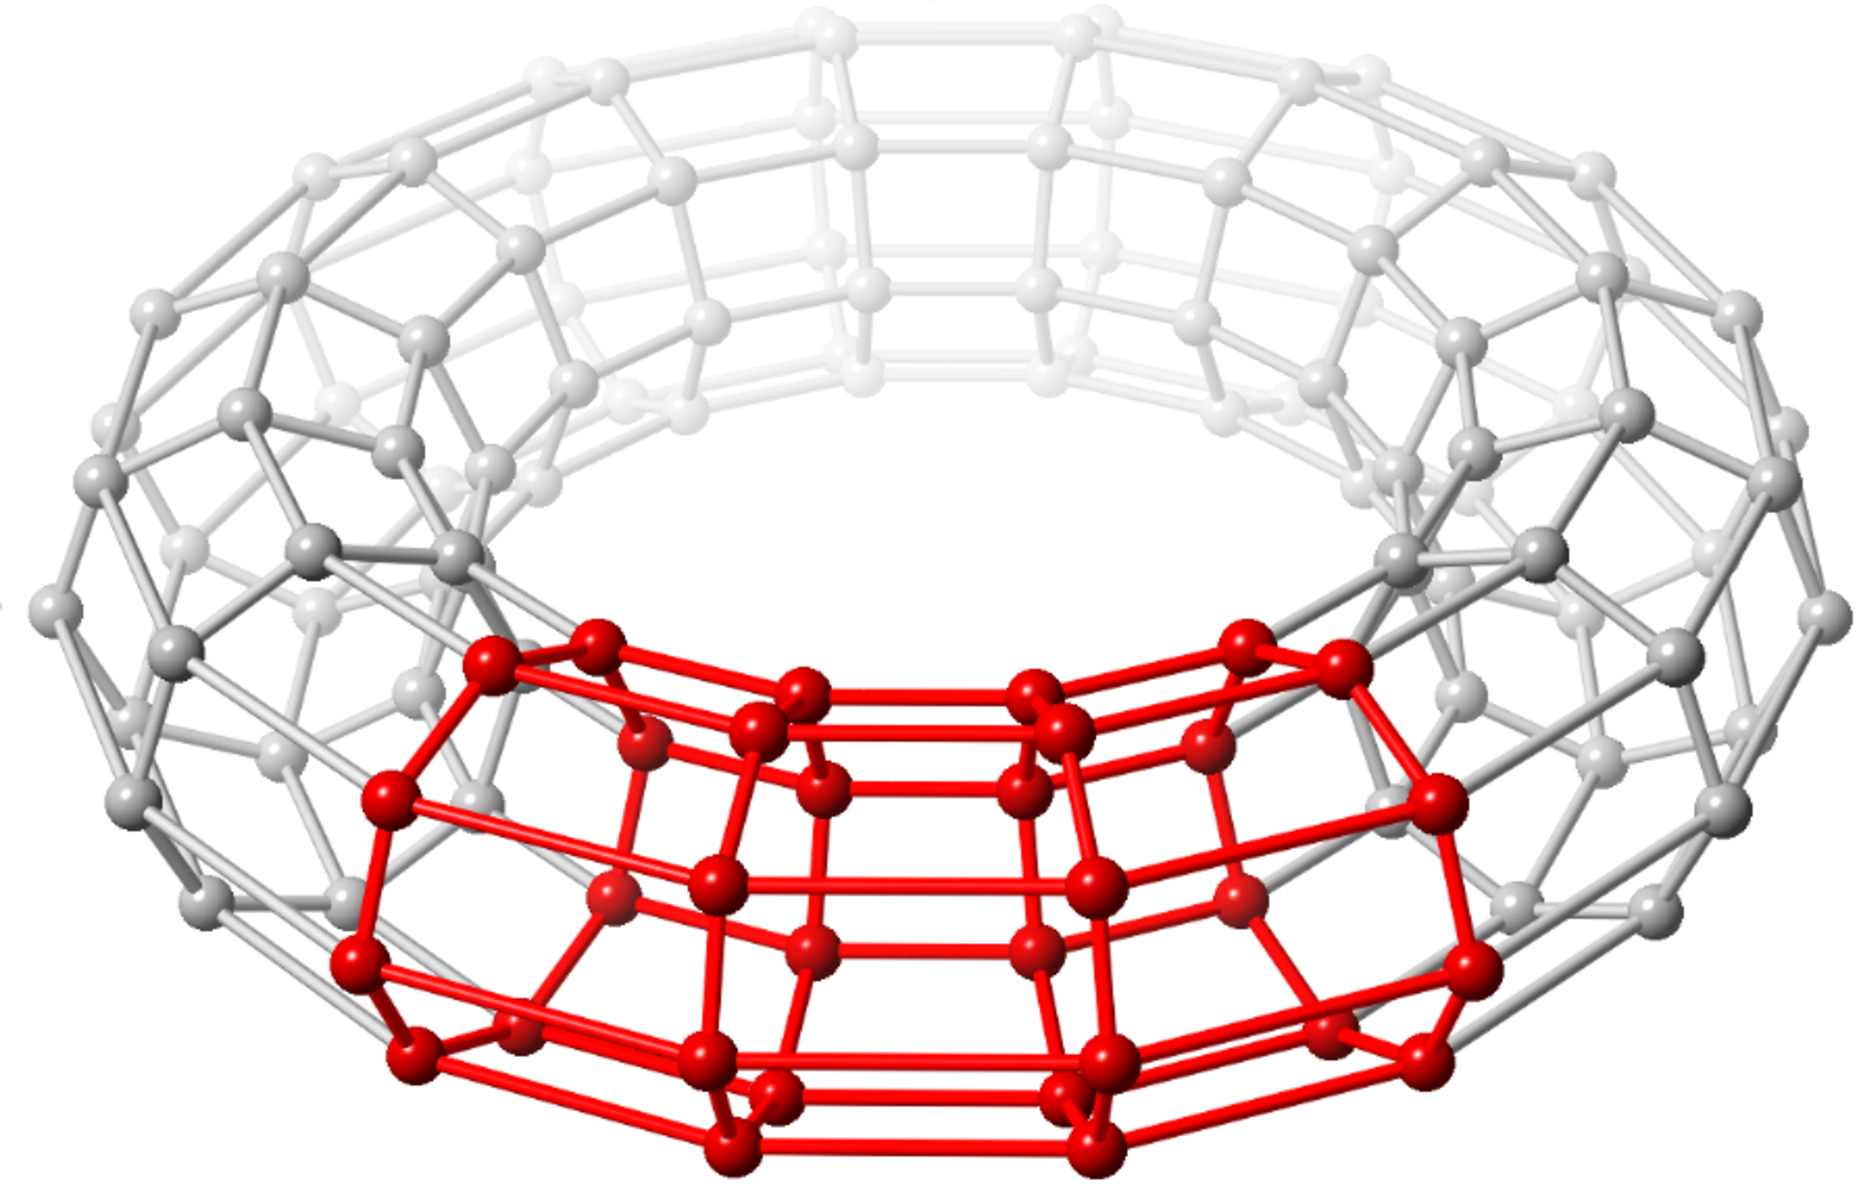
\includegraphics[width=2.1in]{./figs/16x8b.pdf}}
   \end{center}
   \caption{An $8 \times 16$ toroidal lattice.  The width of cylindrical region $A$ (blue) is $x=4$.  The boundary length between region $A$ and its complement is $\ell = 16$. }
   \label{fig:torus}
 \end{figure}
 
{\it Fermions with $\pi$-flux---}
We begin by considering
free spinless fermions on a square lattice, with $\pi$-flux through each plaquette.  We consider a torus of size $L_x$ by $L_y$, and
measure the entanglement % for two different types of region $A$: a $square$ region $A$ containing four corners, and 
using a cornerless cylindrical region $A$ (Fig.~\ref{fig:torus}) with a constant boundary length $\ell = 2L_y$.
We denote the width of region $A$ by $x$.
This system has Dirac points near momentum $k_y=0$ and $k_y=\pi$.  We take anti-periodic boundary conditions in the $x$-direction so that there will be no exact zero mode.  We use exact numerical diagonalization of the single-particle Hamiltonian to compute the entropy.

The entanglement entropy of 2+1-dimensional conformally invariant systems such as this has been argued to be of the form \cite{ryu,ZGV}
\be
S_n \sim {\rm const.}\times \ell /a + \gamma(x/L_x,L_y/L_x),
\ee
where $\gamma$ is a universal scaling function of the dimensionless ratios.
The area-law term proportional to the boundary length $\ell$ depends on the lattice constant $a$, and so the constant is non-universal. A crucial difference
from the result in 1+1D, Eq.~(\ref{1Dcft}), is that $a$ only appears in the area law term.  In contrast, the one-dimensional result can be written as a sum of two terms as
$S_n =C \ln[\sin\big( \frac{\pi x}{L} \big)]+ C\ln[\frac{L}{\pi}] $, where $C=c/(6(1+n))$.
The first term is a universal function of the dimensionless ratio $x/L$, akin to the function $\gamma$ above, while the second term involves the lattice scale, as it diverges with $L$.

To illustrate the absence of such an ``additive logarithm" (a logarithmic divergence depending on $L/a$) in 2D,
we treat this free system as a collection of independent systems in 1D labeled by the momenta $k_y$.
%consider the two-dimensional entropy as a sum of one-dimensional entropies of systems with different momenta, $k_y$.  
The $k_y=0$ mode contributes an additive logarithm $C \ln(L_x)$ to the entropy, while the modes with small $k_y \neq 0$ contribute additive logarithms $C \ln(k_y^{-1})$ \cite{Holzhey,Korepin,Cardy}. Summing over $k_y=2\pi m/L_y$, this gives an entropy $C \big( \ln(L_x)+2\sum_{m=1}^{m \sim L_y} \ln(L_y/2 \pi m) \big)=C\ln(L_x) + 2 C\ln((L_y/2\pi)^{L_y}/L_y!)$, where the factor of $2$ arises from summing over positive and negative $m\neq 0$.  Using Stirlings formula for $L_y!$, one finds that the additive logarithm terms add to $C(\ln(L_x)-\ln(L_y))=C\ln(L_x/L_y)$. This can be absorbed into the scaling function $\gamma$, so that there is no additive logarithm.  A more precise calculation would include the effect of finite $L_x$, but we ignore this since it does not affect the cancellation of additive logarithms. A similar calculation near $k_y=\pi$ leads to a cancellation of the additive logarithm there.


The entropy of a given $k_y$ mode contains, in addition to the additive logarithmic divergence in $k_y$, a universal scaling function $G(x/L_x,k_y x)$.  At $k_y=0$, we see the chord-length scaling $C \ln\sin\big( \frac{\pi x}{L} \big)$ (Fig.~\ref{fig:dirac}), but for $k_y \neq 0$ and for $k_y x$ large, the chord-length scaling disappears and the entropy becomes roughly flat as a function of $x/L$.  In fact, for $L_y=L_x=L$, the lowest $k_y$ mode has a mass $2 k_y=4\pi/L$. This factor of $4\pi\approx 13$ means this mass is rather large, and so the entropy of this mode is flat for a large range of $x/L$.  As a result, for $L_y=L_x=L$, the entropy of the 2D system appears to display 1D chord length scaling over a wide range of $x/L_x$.

 \begin{figure}
   \begin{center}
   \scalebox{1.7}{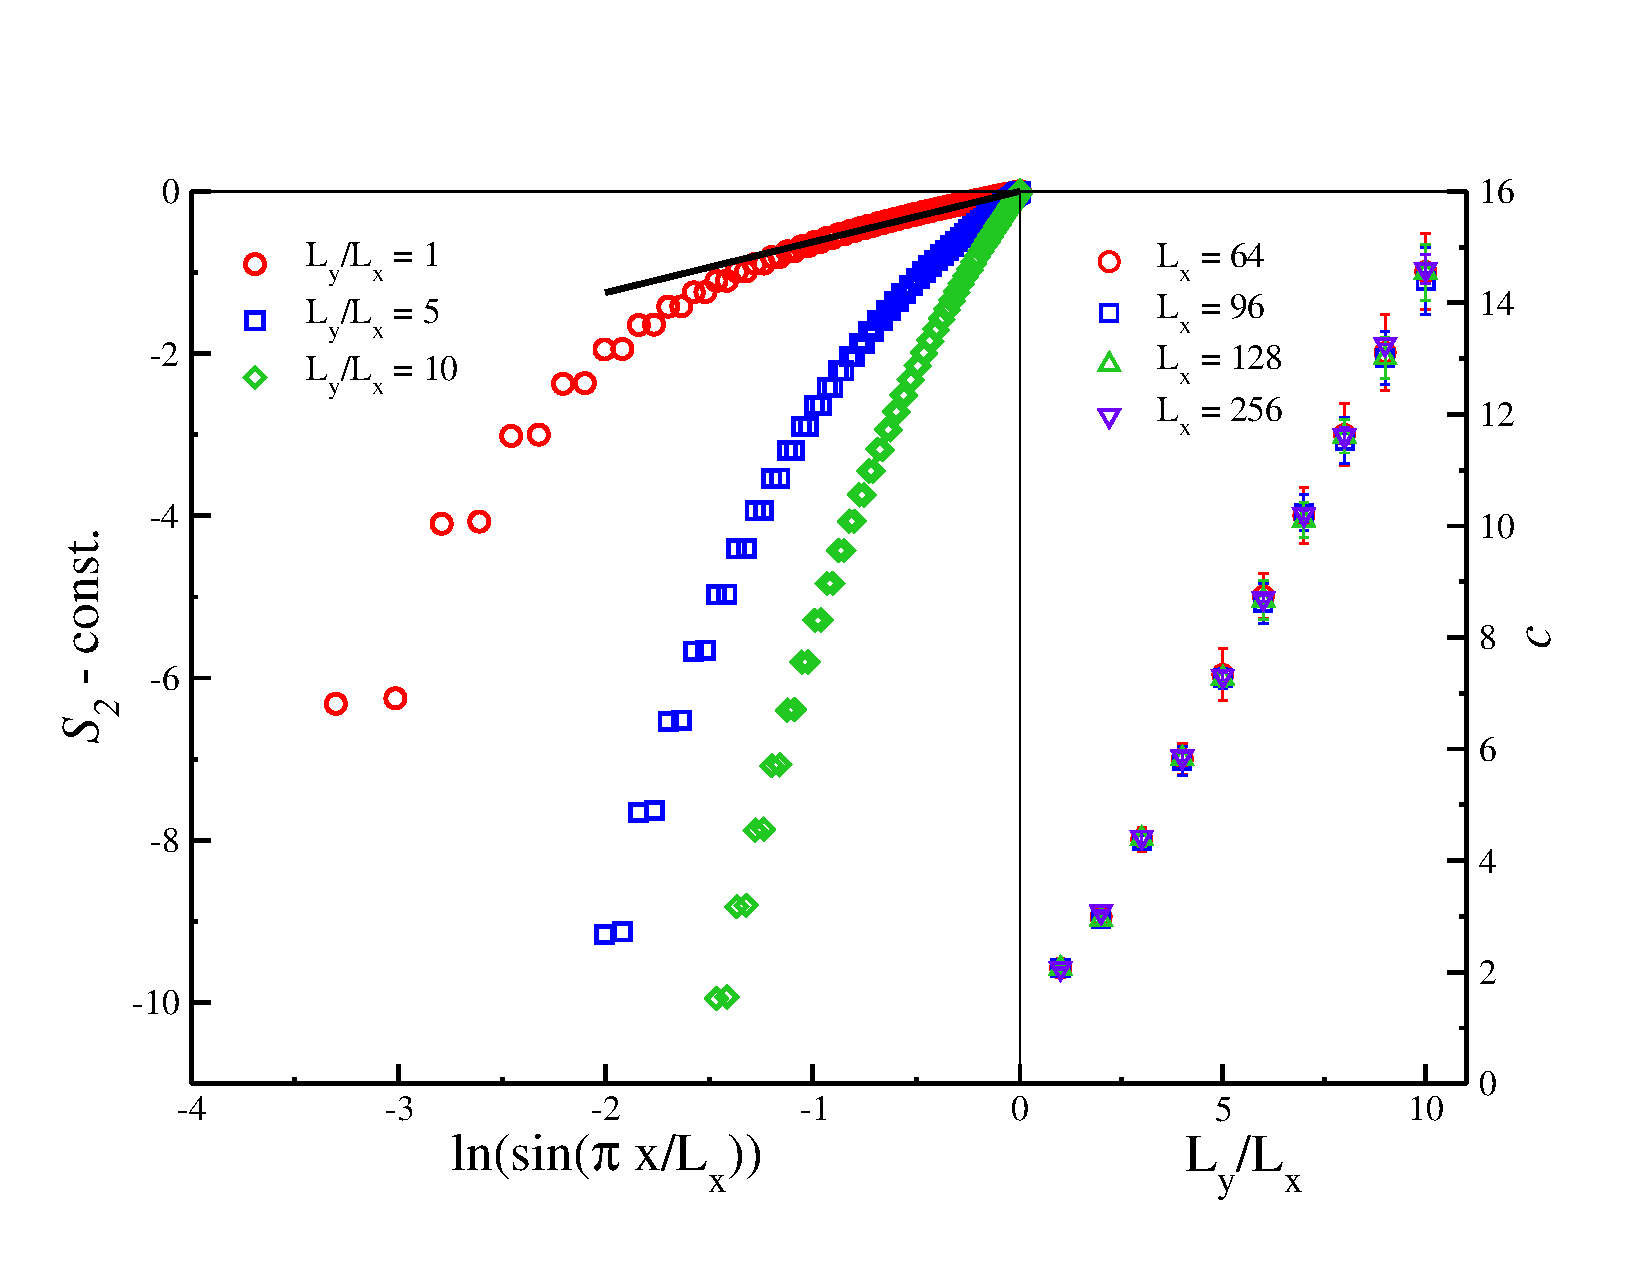
\includegraphics[width=2.1in]{./figs/dirac/fermion.pdf}}
   \end{center}
   \caption{(a) Renyi entropy of $L_x=256$ Dirac fermion model, with an arbitrary constant subtracted off each data set.
    The straight line is Eq.~(\ref{1Dcft}) plotted with $c=2$.
    It is clear that deviations from linearity increase for larger $L_y/L_x$. (b) 
   }
   \label{fig:dirac}
 \end{figure}
 
{\it Quantum Monte Carlo---}
Using QMC techniques we simulate both the
Heisenberg ground state and the RVB
wavefunction in 2D.  The Heisenberg ground state is
projected from a trial state by applying a high power of the
Hamiltonian, $H = \sum_{\langle ij \rangle} {\bf S}_i \cdot {\bf S}_j$, via a QMC method operating in the valence bond (VB)
basis \cite{Sandvik}. 
The RVB wavefunction 
is an equal-amplitude superposition 
$| \Psi \rangle = \sum_{\alpha} | V_{\alpha} \rangle$
of all nearest-neighbor valence-bond states, 
\begin{equation}
|V_{\alpha} \rangle =  \frac{1}{2^{N/4}} \prod_{i=1}^{N/2} \big( | \uparrow_i \downarrow_{j_{\alpha}} \rangle -  | \downarrow_i  \uparrow_{j_{\alpha}} \rangle \big),
\end{equation}
 defined by requiring that each spin $i$ on one sublattice be in a singlet with one of its neighbors $j_\alpha$ \cite{RVB1,RVB2}. The RVB 
Monte Carlo sampling
algorithm does a random walk through the possible states by creating a
defect at some spatial point and propagating it through the system (thereby
rearranging the nearest-neighbor bonds) until the defect reaches the
initial point and its path forms a closed loop \cite{AWSloop}.
If we visualize the Heisenberg ground state in this VB language, then the RVB wavefunction is its largest component, the remainder of the state being equal superpositions, with longer bonds decaying with their length as $1/r^3$ \cite{Sandvik}.  Likewise, the RVB wavefunction is the ground state of a local (but longer-range) Hamiltonian that includes a Heisenberg term \cite{Cano}.


We consider the same geometry as for the $\pi$-flux fermions, with $L_x=L_y=L$ (see Fig.~\ref{fig:torus}).
 \begin{figure}
   \begin{center}
   \scalebox{1}{\includegraphics[width=0.9\columnwidth]{./figs/rvb-heisenberg.pdf}}
   \end{center}
   \caption{ The second Renyi entropy for the N\'eel and RVB states for $L=24$. Note that the entanglement entropy for the RVB splits into two branches, even and odd, which may be related to the existence of topological sectors in the underlying transition graphs.
   %Heisenberg strip data for $L=12,16,\dots,40$ with fits to the function $m\log(\tfrac{L}{\pi}\sin(\tfrac{x\pi}{L}))+h$} for each system size.
   \label{fig:heis_bow} }
 \end{figure}
In Fig.~{\ref{fig:heis_bow}}, we plot QMC results for the Renyi entropy in the N\'eel and RVB states on a $24 \times 24$ torus.  
Several features of the entanglement scaling are clear from this plot.  First, note that the data for the N\'eel state has a significant curvature as a function of $x$.  This curvature was first seen in Ref.~\cite{HeisLog} but not explored in detail (instead, using a fixed $x/L$ a surprising subleading logarithmic term $\propto \ln(\ell)$ was found).
%is present, surprisingly, even with an absence of corners in the region $A$ \cite{MaxLog}.
%N\'eel state, first explored in Ref.~\cite{HeisLog}.  In that work, the presence of an area law term $\propto \ell$ was confirmed, as well as a subleading logarithmic term $\propto \ln(\ell)$ (present, surprisingly, even with an absence of corners in the region $A$).  This subleading term was extracted when the width of the region $A$, $x = L/2$, is equivalent to the ``center'' of each curve in Fig.~{\ref{fig:heis_bow}}.  
There is significant curvature in the $x$ dependence of the RVB wave function as well  (Fig.~\ref{fig:heis_bow}).  However, here there exists a more complicated structure to the entropies: the appearance of two branches (an ``odd branch'' when $x$ is odd, and an ``even branch'' when $x$ is even).  We discuss this branching structure in more detail below.

To capture the $x$-dependent curvature of these wavefunctions, we fit the data with the scaling ansatz
\begin{align}
S_2= a \ell + b\ln(\ell)
+ c(L) \ln \left[{ \sin\left({ \frac{\pi x}{L} }\right) }\right] + d \label{Fit}
\end{align}
motivated by the chord length in Eq.~(\ref{1Dcft}).
We begin by examining the N\'eel state in Fig.~{\ref{fig:heis_lines}}.  For a fixed linear system size $L$, plots of $S_2$ versus $ \ln \left[{ \sin\left({ \frac{\pi x}{L} }\right) }\right] $ would yield a straight line if Eq.~(\ref{Fit}) were obeyed perfectly.  The plots indeed are quite close to straight lines for a fixed $L$.

The second Renyi entropy therefore displays at the very least an effective chord-length dependence over a large range of $x$ for the square torus. It is possible that the apparent chord-length scaling of this 2D system is not perfectly obeyed in the thermodynamic limit, and that this fact is manifest in slight deviations from straight-line behavior in Fig.~{\ref{fig:heis_lines}}(a).
This would be a similar scenario to the deviation from chord-length scaling observed for $\pi$-flux fermions in Fig.~\ref{fig:dirac}.  
However, it is difficult to draw a firm conclusion regarding the statistical significance of any deviation from Eq.~(\ref{Fit}) scaling in our
present data, due to limited system sizes and stochastic error.

 \begin{figure}
   \begin{center}
   \scalebox{1}{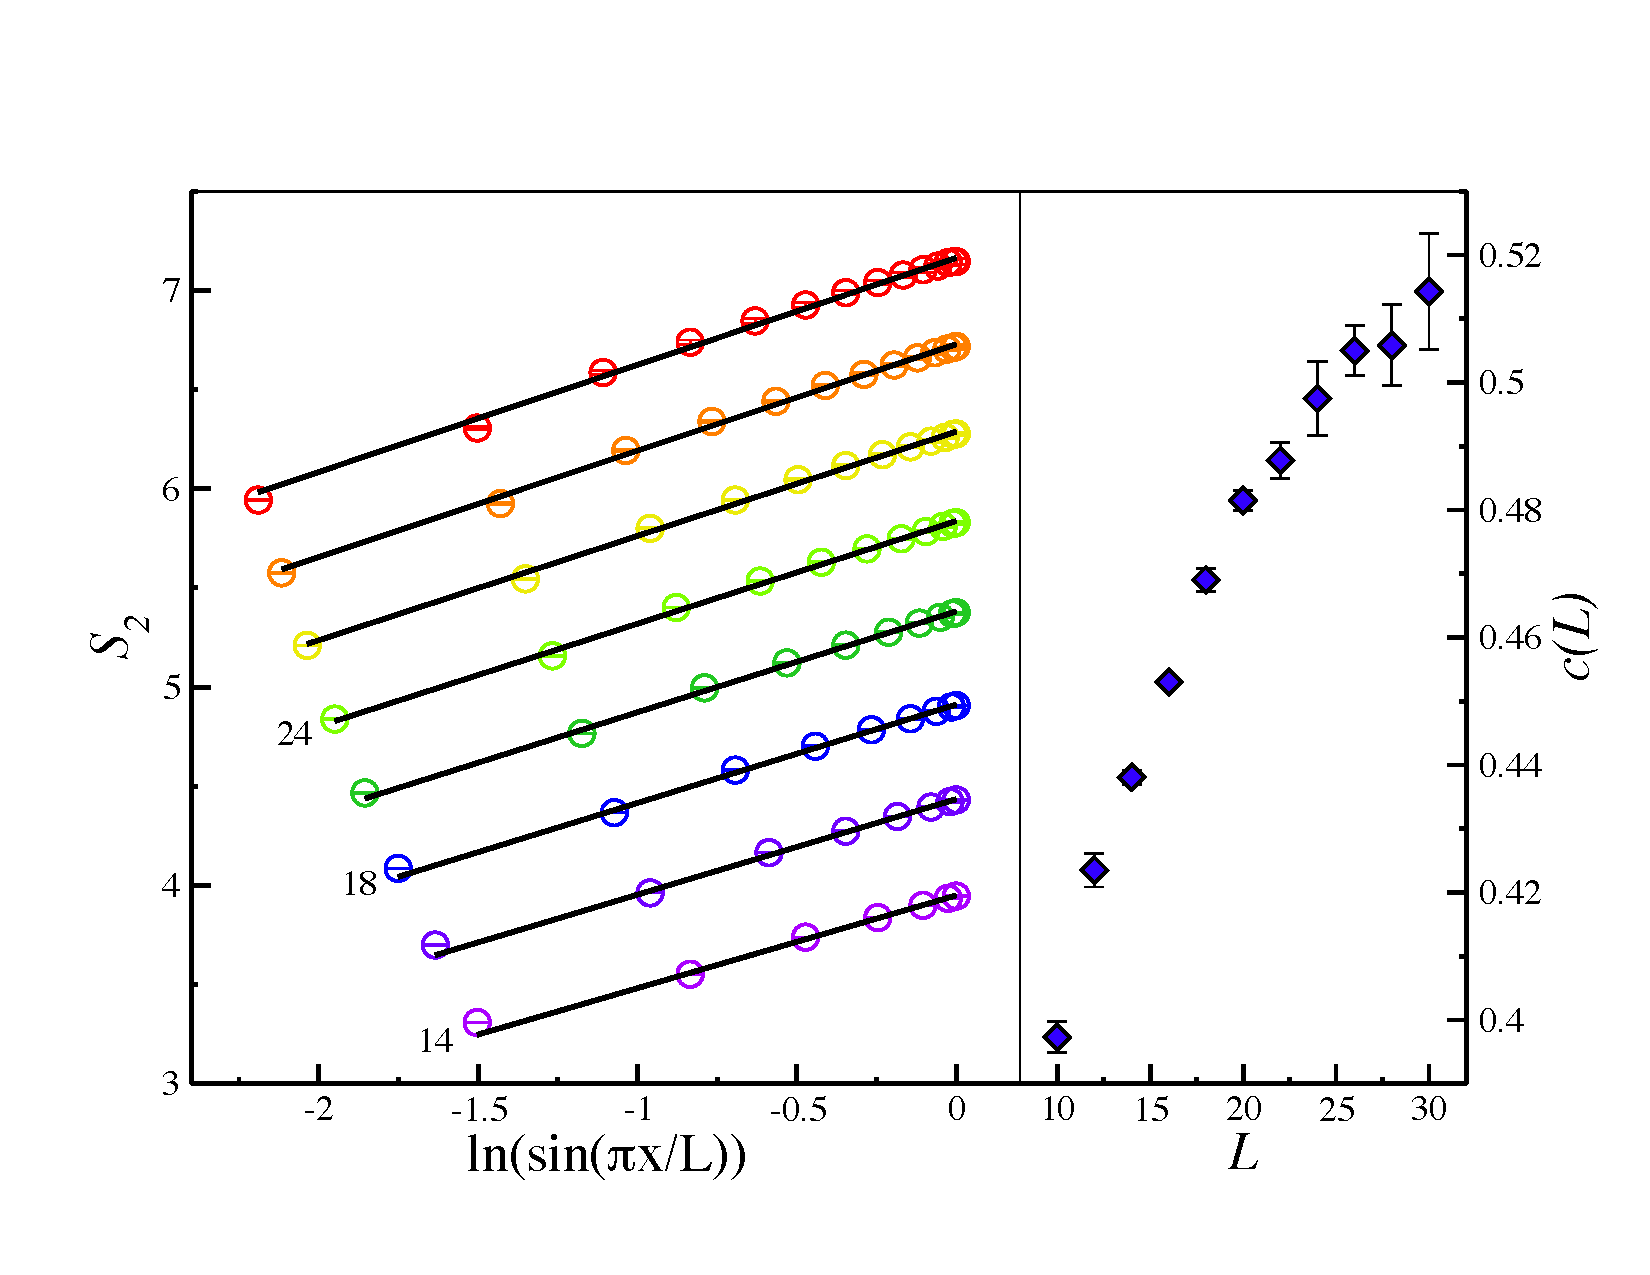
\includegraphics[width=\columnwidth]{./figs/heis.pdf}}
   \end{center}
   \caption{(a)Heisenberg data and linear fits (excluding the first two data points on the left) for $L=14,16,\dots,30$ plotted in terms of the log of the ``chord-length", $\ln\left[\sin \frac{\pi x}{L}\right]$.
   (b) Slopes of the fits, $c(L)$, exhibit a strong dependence on the system size, $L$.
   }
   \label{fig:heis_lines}
 \end{figure}

%In fact, as is visible in the largest $L$ considered, there is a slight deviation of the straight-line fits for small $x$.  
We can however further examine the deviation from conformal-style scaling by examining the universality of the 
coefficient of the chord-length in the N\'eel state.
To do this, we extract the $L$-dependence of the coefficient $c(L)$ in Eq.~(\ref{Fit}).  As illustrated in Fig.~\ref{fig:heis_lines}(b),
the coefficient does not approach a constant for the system sizes that we have studied, but rather has some functional dependence on $L$.
This functional dependence is apparently sub-linear.  It is interesting to speculate that $c(L) \sim L^p$ with $p\leq1$.  A rigorous analysis of the data along this lines is impossible however within the current
accuracy of our QMC simulations.

%It is clear in that this form gives an excellent fit to the data for all $x$ and $L$, providing strong evidence for the presence of the chord length.  We can analyze the fits further by examining the dependence of the coefficients on system size $L$.  Most interestingly, we observe the coefficient of the chord-length increasing with $L$, as illustrated in the inset of Fig.~{\ref{fig:1}}.

 \begin{figure}
   \begin{center}
   \scalebox{1}{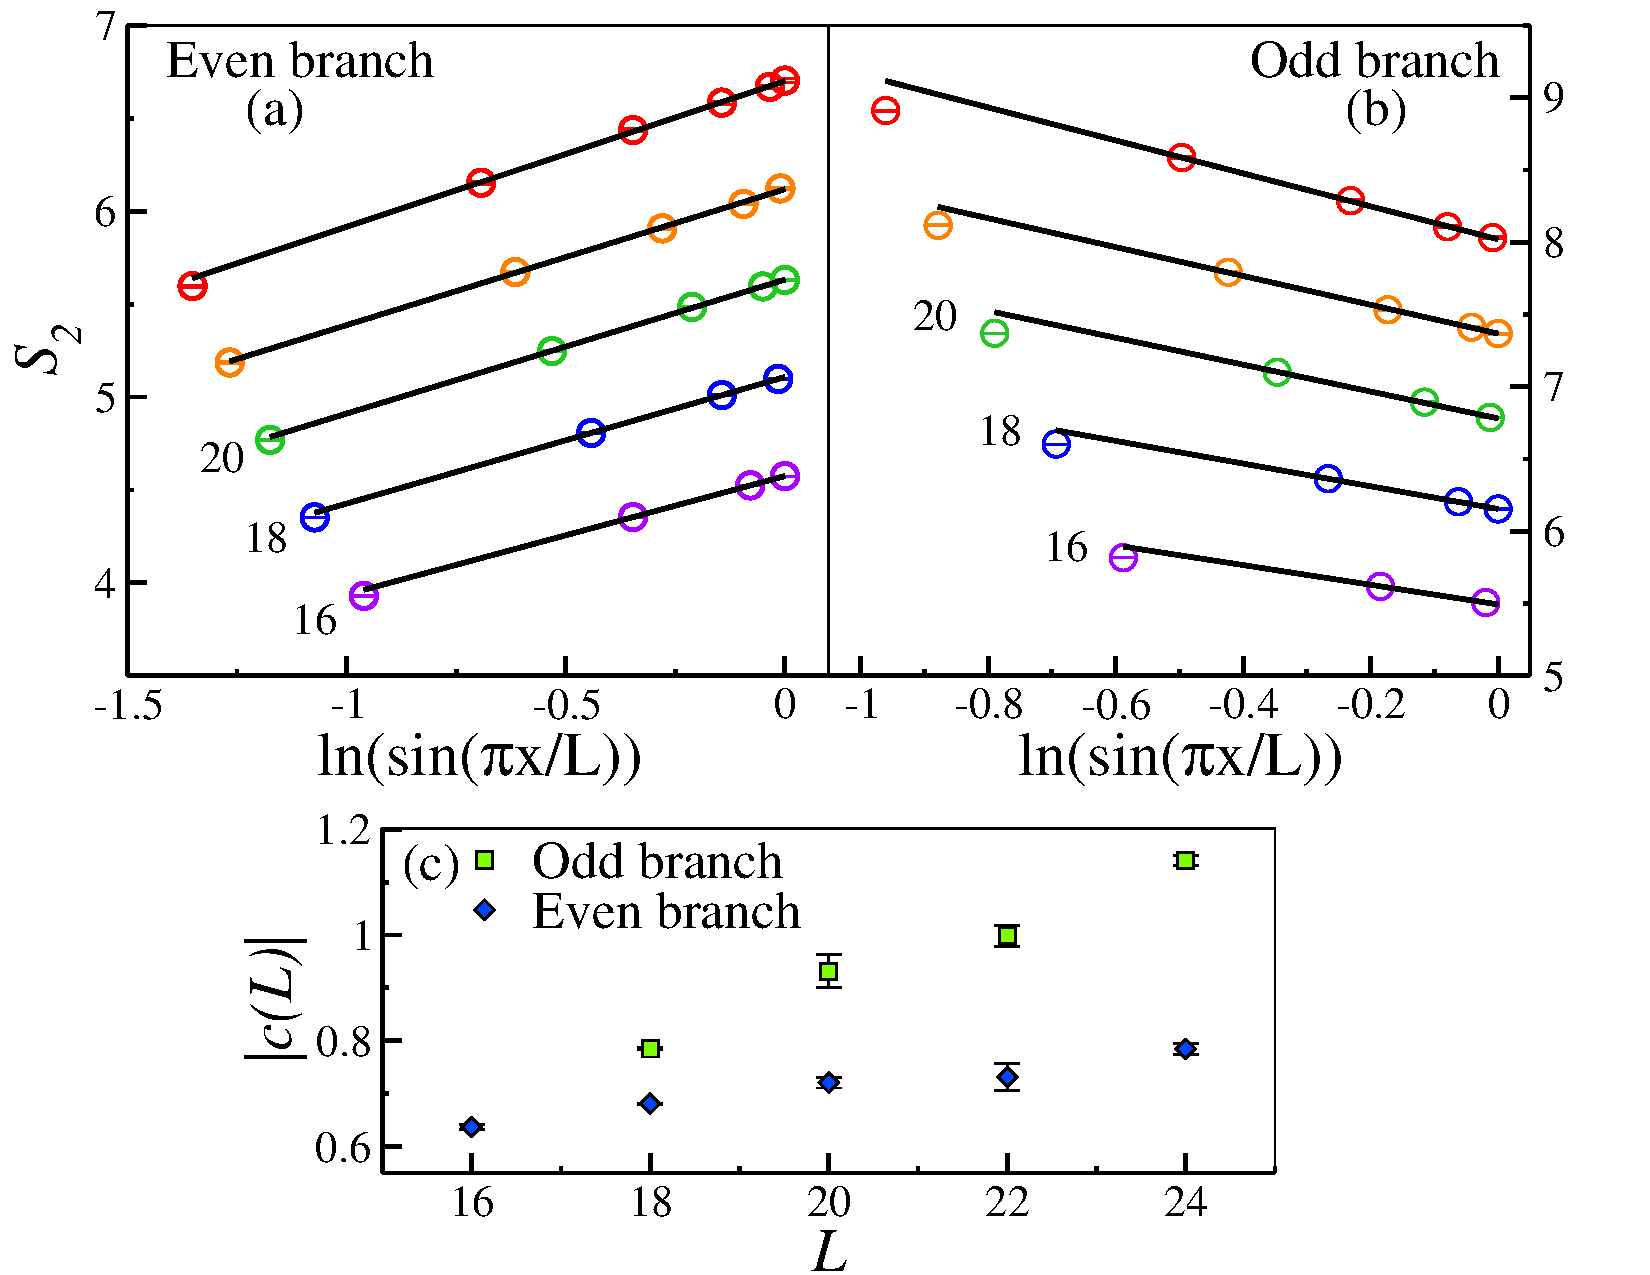
\includegraphics[width=\columnwidth]{./figs/rvb/rvb-bow.pdf}}
   \end{center}
   \caption{(a) Even and (b) odd branches of the second Renyi entropy plotted against the log of the ``chord-length". We exclude $x=1,2$ data from the plots, as there is some crossover behavior observed in Fig.~\ref{fig:heis_bow}. (c) The slopes, $c(L)$, as a function of the system size, $L$. As with the Heisenberg, there is a strong dependence on $L$.}
   \label{fig:2}
 \end{figure}

We next examine the scaling of the Renyi entropy in the RVB wavefunction, illustrated in Fig.~{\ref{fig:2}}.  
As discussed in Fig.~\ref{fig:heis_bow}, a striking two-branch structure exists, depending on whether the distance $x$ is even or odd.
The presence of the two branches presumably is related to the fact that correlators in the RVB state have a pronounced even-odd dependence. Moreover, simple counting arguments of prototypical valence-bond configurations in the (0,0) topological sector \cite{RVB1,RVB2} show that the number of valence bonds crossing from region $A$ to region $B$ alternates strongly with $x$.  From this $L=24$ data there is a clear $x$-dependent curvature in each branch: this can be analyzed more closely by examining each branch individually and attempting fits of the form Eq.~(\ref{Fit}).  

In Fig.~{\ref{fig:2}}(a) and (b), it is clear that fits to the scaling ansatz to both branches are quite accurate when the extremal values of $x$ are excluded.   Unfortunately, due to the two-branch structure of the Renyi entropy in the RVB wavefunction, each curve on this plot has essentially half the usable data compared to the analagous Heisenberg results in Fig.~\ref{fig:heis_lines}.  Nonetheless, we can attempt to extract the size-dependence of the coefficient $c$ in a similar manner.  The result (Fig.~\ref{fig:2}(c)) shows that a significant $L$-dependence again seems to exists in the RVB wavefunction.  This may again suggest that, although the fit of individual $L$ data to a chord-length scaling is consistent within the accuracy of our data, subtle corrections to this form may come into play in the 2D thermodynamic limit.

{\it Discussion---} We have studied the Renyi entanglement entropy in the ground state of three gapless systems on $L_x\times L_y$ toroidal lattices, where the subregion $A$ is a cylinder of length $x$.  We have  
demonstrated that it contains a universal subleading scaling term $\gamma(x/L_x,L_y/L_x)$, which depends on bulk quantities, namely the dimensionless aspect ratios of the subregion and the lattice linear dimensions.  
Note that while numerical measurement of topological entanglement entropy\cite{LW,KP} has been used to probe topological properties of {\it gapped} phases\cite{isakov}, the universal subleading term considered here means that a measurement of topological entanglement entropy in a {\it gapless} phase could give either a zero or non-zero result, even without any topological aspects of the phase (though measurements in the $U(1)$ superfluid phase yielded a vanishing number\cite{isakov}).
%The presence of the universal term shown here means that in principle the topological entanglement entropy\cite{LW,KP} could be non-zero in a {\it gapless, non-topological} phase such as a $U(1)$ superfluid. This has yet to be seen; for example, the measurement of Ref.\ 
% \onlinecite{isakov}  in the Bose-Hubbard model on the Kagom\'e lattice yielded a non-zero value only in the {gapped, topological} phase.  
Interestingly, just as strong sub-additivity constrains the sign of the Levin-Wen entropy \cite{LW}, it also implies that for fixed $L_x,L_y$ that $\gamma$ is a concave-down function of $x$.

Our quantum Monte Carlo simulations of the Heisenberg N\'eel ground state and the short-range RVB wavefunction with $L_x=L_y=L$ show an almost-perfect dependence of $\gamma$ on the chord length $\sin(\pi x/L)$.
It appears that the coefficient of this term is not a universal constant, however, which might suggest that care must be taken the order of limits with which the thermodynamic limit is approached. A study of the crossover from one to two dimensions might also illuminate this issue further.  Further evidence that the true 2D scaling function might be more complicated than the chord-length form is given by the scaling of gapless Dirac fermions in the $\pi$-flux phase. Here we have argued that such scaling is superseded by a sum over transverse modes, leading to a different (unknown) functional form in 2D.  Further,  spontaneous symmetry breaking in the Heisenberg model may complicate measurement of the entanglement entropy, and current simulations are unable to completely characterize the scaling behavior of these terms in the Heisenberg and RVB models at large sizes.

Regardless of the precise functional form of $\gamma(x/L_x,L_y/L_x)$, its general existence in gapless wavefunctions in 2D would have some profound consequences.  
Most immediate may be the complications that arise while attempting to use entanglement as a probe to detect gapless spin liquids, since it gives a clear non-zero signature in the quantities used to define the topological entanglement entropy \cite{KP,LW}.
%Most immediate may be it's complication of attempts to use entanglement to detect gapless spin liquids,
%since it gives a clear non-zero signature in the quantity used to define the topological entanglement entropy \cite{KP,LW}.
In addition, the similarity of the scaling function to a chord-length (present in 1D conformally invariant systems) 
raises the tantalizing possibility that our results will prove useful in characterizing higher-dimensional critical points.
Indeed, since the search for a $c$-theorem \cite{Zamo} valid in higher dimensions is of intense interest across several disparate field of physics (see e.g.\ \cite{Cardy88,ryu,Myers,Komargodski}),
we hope our results inspire a broader examination of the existence of this scaling term in two-dimensional gapless states.

{\it Acknowledgments---} 
The authors thank A.~Del Maestro, I.~Klich, K.~Intriligator,  M.~Metlitski, E.G.~Moon, R.~Myers and A.~Sandvik for enlightening discussions. 
R.G.M. would like to acknowledge the support of Microsoft Station Q for hospitality during a visit.
This work has been supported by the Natural Sciences and Engineering
Research Council of Canada (NSERC), and by the US NSF via grants DMR/MPS-0704666 and DMR/MPS1006549.  Simulations were performed on the computing facilities of SHARCNET.


\bibliography{rvb_bib}

\end{document}
